\documentclass[tikz]{standalone}
\usepackage{pgfplots}
\usepackage{mathptmx}
\usepackage{ctex}
% \pgfplotsset{compat=1.16}
\begin{document}
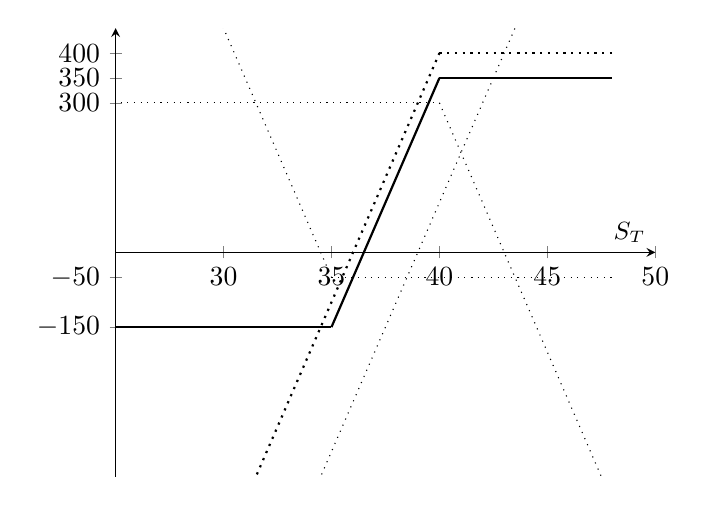
\begin{tikzpicture}
    \begin{axis}[
        axis lines = middle,
        xlabel = {$S_T$},
        ymin=-450, ymax=450,
        xmin=25, xmax=50,
        scaled x ticks=false,
        % xtick={13560,13910,14085},
        ytick={(\Kp-\Pp+\Pc-39)*100, -50,0,300, 350,400},
        % width=10cm,
        % height=7cm,
        % axis equal,
        label style={font=\small}
    ]
    % 定义参数
    \def\Pc{3}  % 期权费
    \def\Pp{0.5}
    \def\Kc{40}
    \def\Kp{35}
    
    % 绘制看涨期权到期收益曲线
    \addplot[domain=25:48, dotted] {(x-39)*100};
    \addplot[domain=\Kc:48, dotted] {(\Kc-x+\Pc)*100};
    \addplot[domain=0:\Kc, dotted] {\Pc*100};
    \addplot[domain=0:\Kc, thick, dotted] {(x-39+\Pc)*100};
    \addplot[domain=\Kc:48, thick, dotted] {(40-39+\Pc)*100};
    \addplot[domain=0:\Kp, dotted] {(\Kp-x-\Pp)*100};
    \addplot[domain=\Kp:48, dotted] {(-\Pp)*100};

    \addplot[domain=0:\Kp, thick] {(\Kp-\Pp+\Pc-39)*100};
    \addplot[domain=\Kp:\Kc, thick] {(\Pc-\Pp+x-39)*100};
    \addplot[domain=\Kc:48, thick] {(\Pc-\Pp-39+\Kc)*100};
    
    \end{axis}
\end{tikzpicture}

\end{document}